% !TEX root = main.tex

\section{Introduction}


We study the problem of non-stationary spatial correlations. We extend on our previous work on crime rate inference across communities~\cite{WKGL16}. We select Chicago as the target of study for the following reason. Chicago has more homicides and non-negligent manslaughter rates (15.2) per 100,000 residents than New York (4.0) and Los Angeles (6.5) according to the FBI crime statistics for 2013 and has experienced no decline in the past decade compared to the other two large cities, which have been on a slow declining slope \cite{crime-stats}.


Traditionally, researchers have used demographic information based on Decennial Census (e.g., population poverty level, socioeconomic disadvantage, racial composition of population) to estimate the crime rate in a community~\cite{GrSa09}. Existing studies also highlight the importance of geographical influence~\cite{Ans02} in estimating crime rates, i.e., the crime in the nearby communities can be propagated to the focal community.
 
\begin{figure}[t]
\centering
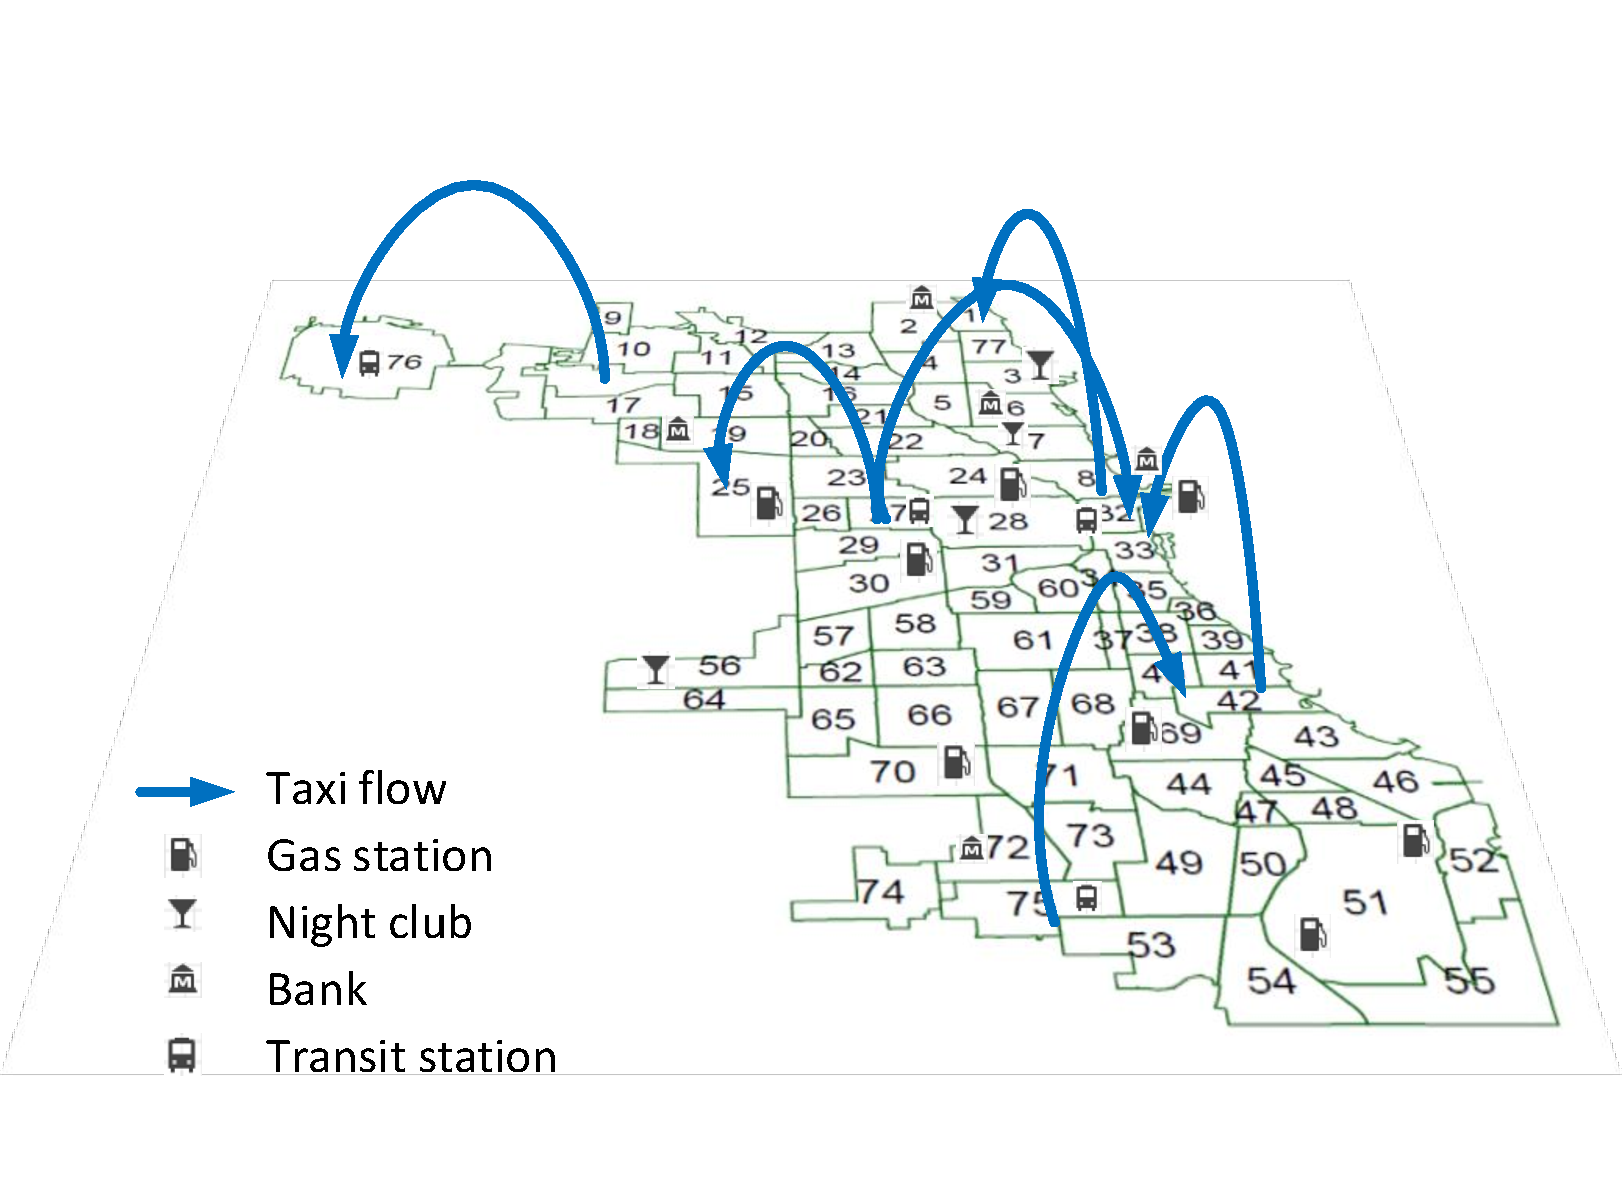
\includegraphics[width=0.8\linewidth]{fig/demo-kdd16.pdf}
\caption{An illustration of various types of features we use in Chicago. The POI distributions across community areas profile the region functionality. The taxi flows connect non-adjacent regions and act as ``hyperlinks'' on the space.}
\label{fig:demo}
\vspace{-3mm}
\end{figure}

Recently, big data reflecting city dynamics have become widely available~\cite{ZCWY14}, e.g., traffic flow, human mobility, social media, and crowd-generated Points-Of-Interest (POI). As shown in Figure~\ref{fig:demo}, such newer types of big data could provide new insights to advance our understanding of traditional socioeconomic urban problems, such as the crime rate inference problem we focus on in this chapter. In particular, we propose to study two newer types of urban data: POI and taxi flow. 

\textbf{POI data.} POI data provide venue information such as GPS coordinates, category, popularity, and reviews. These POIs mostly belong to categories such as food, shop, transit, education, etc. Recent studies have shown that using such categorical information of POIs are helpful to profile neighborhood functions~\cite{YZX12}. Such neighborhood functions could further help us predict crime rate (e.g., communities with less education or entertainment facilities may have a higher rate of crime).

\textbf{Taxi flow data.} A huge amount of taxi flow data reflect important information about how people move across neighborhoods in the city. In previous studies, when using geographical influence~\cite{Ans02}, scientists assume that a community is affected by other spatially proximate communities. However, even if two communities are distant in geographical space, they could be strongly correlated if many people frequently travel between these two communities~\cite{GGM14}. We hypothesize that taxi flows may be considered as ``hyperlinks'' in the city that connect different areas and we use such data to estimate crime rates. 



As an extension to Chapter 2, we investigate models that incorporate geographic heterogeneity; that is, we do not expect the same features to have the same relation to crime in every location because crime incidents in different regions may be associated with different social-economic factors.
In fact, there are several neighborhoods where negative binomial model gives poor prediction. This tells us that a global model such as the negative binomial model, which assumes a constant correlation between crime and observed features, would not yield accurate estimates. Therefore, we further propose to employ a graphically weighted regression approach to capture the non-stationary property of crime. The intuition behind this strategy is to train many local models instead of one global model to predict the crime. The geographically weighted regression is a useful framework on how to pick samples and weight them for local model training. We thus apply geographically weighted regression in combination with negative binomial model, and the experiments show further improvements over the global model.


In summary, the contributions of this chapter are:  1) We study an old but important crime inference problem by utilizing new urban data: POIs and taxi flows. We provide detailed discussions of how to construct features, tests of different combinations of features, and the theoretical interpretations of the result from a social scientist (a co-author in the paper). 2) We find that utilizing these new types of big urban data improves the crime rate inference. 3) We employ a geographically weighted regression framework to capture the non-stationary property of crime. 4) We conduct a systematic comparison between various regression models. The geographically weighted negative binomial model has significantly better performance, and could serve as a new baseline for future crime inference problems.

The rest of this chapter is organized as follows. The crime inference problem is formulated in Section \ref{ch5-sec:overview}. We discuss the inference model in Section \ref{ch5-sec:model}. The Section \ref{ch5-sec:experiment} presents the quantitative evaluation results on real data. We review the related work in Section \ref{ch5-sec:related-work}.  Finally, we conclude this chapter in Section \ref{ch5-sec:conclusion}.

